\documentclass[11pt]{article}
\usepackage[margin=1in]{geometry}
\usepackage{graphicx,booktabs,amsmath,hyperref}
\sloppy
% generated by ios/tools/plot_tests.py
\newcommand{\iosPassed}{17}\newcommand{\iosFailed}{0}
\newcommand{\iosTable}{launch to studio and engine found & 4.21 & 4.18 to 4.23 & s & 2 \\
servo samples reaching the plots & 32.95 & 32.46 to 33.44 & Hz & 2 \\
tap to seated & 0.80 & 0.80 to 0.81 & s & 2 \\
tap to standing & 0.70 & 0.68 to 0.72 & s & 2 \\
left stick forward 3 s: distance ahead & 1.21 & 1.20 to 1.21 & m & 2 \\
left stick back 3 s: distance ahead & -1.29 & -1.31 to -1.26 & m & 2 \\
left stick half forward 3 s: distance ahead & 0.49 & 0.49 to 0.49 & m & 2 \\
left stick right 3 s: distance to the left & -0.64 & -0.64 to -0.64 & m & 2 \\
\quad heading change meanwhile & 83.00 & 83.00 to 83.00 & deg & 2 \\
left stick left 3 s: distance to the left & 0.68 & 0.65 to 0.71 & m & 2 \\
\quad heading change meanwhile & -81.00 & -81.00 to -81.00 & deg & 2 \\
right slider clockwise 1.5 s: heading change & -74.50 & -76.00 to -73.00 & deg & 2 \\
\quad distance moved meanwhile & 0.02 & 0.02 to 0.02 & m & 2 \\
right slider anticlockwise 1.5 s: heading change & 61.50 & 57.00 to 66.00 & deg & 2 \\}
\newcommand{\iosDrive}{1 & 0.20 & 0.70 & 0.30 & 0.98 \\
2 & 0.30 & 0.97 & 0.50 & 1.65 \\
3 & 0.40 & 1.15 & 0.70 & 2.09 \\
4 & 0.50 & 1.29 & 0.80 & 2.36 \\
5 & 0.60 & 1.55 & sprint & 3.99 \\}

% generated by ios/tools/bench_stick.py
\newcommand{\iosStick}{forward & 0.25 & 0.10 & 0.14 & m/s \\
forward & 0.50 & 0.20 & 0.24 & m/s \\
forward & 0.75 & 0.30 & 0.34 & m/s \\
forward & 1.00 & 0.40 & 0.41 & m/s \\
backward & 0.25 & -0.10 & -0.12 & m/s \\
backward & 0.50 & -0.20 & -0.23 & m/s \\
backward & 0.75 & -0.30 & -0.36 & m/s \\
backward & 1.00 & -0.40 & -0.45 & m/s \\
sidestep right & 0.25 & -0.07 & -0.07 & m/s \\
sidestep right & 0.50 & -0.14 & -0.14 & m/s \\
sidestep right & 0.75 & -0.21 & -0.21 & m/s \\
sidestep right & 1.00 & -0.28 & -0.27 & m/s \\
turn clockwise & 0.25 & -0.17 & -0.35 & rad/s \\
turn clockwise & 0.50 & -0.35 & -0.55 & rad/s \\
turn clockwise & 0.75 & -0.52 & -0.73 & rad/s \\
turn clockwise & 1.00 & -0.70 & -0.98 & rad/s \\}
\newcommand{\iosCombo}{(0.24, -0.14, -0.35) commanded, (0.28, -0.14, -0.37) measured}
\newcommand{\iosStickFalls}{0}


\title{Duck for iPhone: one screen for the Microduck's state, calibration and driving}
\author{Microduck replication (Feetech HD1910)}
\date{2026-11-17}

\begin{document}
\maketitle

\begin{abstract}
A SwiftUI app (iOS 26, Liquid Glass) that puts the servo studio and the Duck Live engine on a phone. The top bar
chooses what it talks to, the real duck (default) or the simulated one, and offers Connect while the real one is
not connected. Two modes: \emph{Duck} (battery, which servos and sensors answer, live plots, the studio's calibration flow, zero / test / gains per servo)
and \emph{Play} (a left stick for translation, a right slider for turning, a speed slider, sit, run, jump, flip, 27
emotions). It finds both servers on the Wi-Fi by itself. Tested in the iOS simulator with XCUITest against a mock
servo bus and the real engine: \iosPassed{} test runs passed, \iosFailed{} failed. It is installed on an iPhone but
has not been exercised there. With the real duck selected, Play drives the policies trained for this duck, which
run on the duck (its \emph{pilot}, in Setup mode), with the same pad as the simulated duck, and plays the duck's
animations on its head, beak and speaker; in Run mode it drives the factory runtime (Pollen's control daemon)
instead. Both were tested against stand-ins (for the pilot: the duck's real pilot code and policy pack with a still
IMU and no servo). The app has not moved the real duck: there it was checked only as far as the factory runtime's
greeting and health report, with no joint powered.
\end{abstract}

\textbf{Keywords:} teleoperation interface, SwiftUI, SceneKit, Bonjour, bipedal robot, servo calibration.

\section{Overview}
Two servers already exist on the Mac. \texttt{firmware/studio.py} talks to the real servos and, over SSH, to the
duck's computer and its sensors. \texttt{app/server.py} runs the policies on a MuJoCo plant at 50~Hz
(\texttt{docs/duck\_live\_app.pdf}). Both listened on 127.0.0.1 only. The app adds no third server: each gained a
\texttt{--lan} flag (\texttt{ios/lan.py}) that listens on every interface and registers a Bonjour service
\texttt{\_microduck.\_tcp} whose TXT record says which server it is (and, for the engine, its WebSocket port and
token). The phone browses for that type, so nothing is typed and there is no setup screen.

\textbf{Straight to the duck.} The studio can also run on the duck's own computer (\texttt{studio.py --duck
--lan}, put there by \texttt{firmware/duck\_serve.sh} as a systemd user service that starts at every boot, with
no root needed): it uses the duck's sensors and servo port in-process instead
of over SSH, announces itself through Avahi, and never takes the servos from the duck's runtime unasked. The app
looks for it in three ways, with nothing typed: over Bonjour; every 3~s (every second while it has no studio) at the address where it last answered and
at the duck's own addresses (\texttt{radxa-zero3.local} on the Wi-Fi, \texttt{10.42.0.1} on its hotspot); and, while
nothing is found, every 15~s (and at once when Connect is tapped) by asking port 8770 of all 254 addresses of each
private /24 network the phone has an address on, in parallel with a 1.2~s timeout. In a check on the simulator, a stand-in studio started on the
Mac's Wi-Fi address with no announcement was found 7.5~s later (one trial). A real (not mock) studio that
answers is used in preference to one announced by the Mac, and dropped again after three missed polls. Once a
real duck answers, the app connects its computer and servo bus by itself (retried every 2~s until both are up); a
switch turned off by hand stays off, and in Run mode the bus is left to the runtime. The sweep
assumes a /24 network; on a larger one it covers only the phone's own last-octet range. Because a Mac studio's agent and the duck's studio can both be on the servo
port, the port's packet exchange now holds an advisory file lock (\texttt{flock}), one packet at a time.

The target switch maps onto those servers: \emph{Duck} is the studio, \emph{Sim} is the engine. Connect starts the
link to the duck's computer and then opens the servo bus (through the duck if it offers its port, else the first
adapter). With the real duck selected, Play drives the duck's own policies in Setup (Section~\ref{sec:pilot})
and the factory runtime in Run (Section~\ref{sec:runtime}).

The app follows the studio page feature for feature, through the studio's own routes and state; nothing is
recomputed on the phone:
\begin{itemize}\itemsep0pt
\item \textbf{Battery.} The studio's estimate (median servo supply voltage on a two-cell lithium-ion curve,
\texttt{firmware/README.md}) in the top bar, orange under 40\,\%, red under 15\,\% with a warning. It is an
estimate from voltage, not a fuel gauge.
\item \textbf{Temperature and status.} The bar shows the duck computer's processor temperature (the hottest
servo's when the computer is not linked); the panel shows both, with the hottest servo's ID, the computer's host
name and load, and the studio's address. Orange / red at 75 / 90~$^\circ$C for the processor (the RK3566 throttles
from about 85 and shuts down near 115) and at 55 / 65~$^\circ$C for a servo (the HD1910's own protection is 70);
going red raises a warning once per excursion. These limits are this app's choice, not measured on this duck.
\item \textbf{Calibration.} Calibrate (needs all 15 servos) makes every servo limp; Hold switches the torque of all
of them; a joint is trimmed from its card with the slider or the 0.2$^\circ$ nudges; Save records the home pose,
Cancel changes nothing. Once calibrated the card shows the joint angle.
\item \textbf{IMU calibration.} In the IMU window, as in the studio: \emph{1 Upright} (the duck upright, trunk
level) then \emph{2 Beak up} (on its back, beak straight up), each held still. Gravity in the first pose gives the
trunk's up axis in the chip's axes, in the second its front axis (squared against the first; the studio refuses
poses less than 60$^\circ$ apart); left is their cross product. Step 2 is offered only after step 1 and writes the
calibration. Four more buttons turn the result: the front a quarter turn to the left, or a half turn about the
front (X), left (Y) or up (Z) axis. The mathematics is the studio's (\texttt{firmware/studio.py},
\texttt{imu\_cal}, \texttt{imu\_turn}); the app only calls it.
\item \textbf{Setup / Run.} Who has the duck's servos and sensors: the studio, or the duck's own runtime.
\item \textbf{Voice.} The six sounds of the duck's voice bank.
\item \textbf{Flip, live pose, camera.} Flip reverses a calibrated joint's direction. Once calibrated, the 3-D
duck takes the real joint angles (each body moved by the joints that carry it, trunk first, about their baked
axes). The camera picture is turned a quarter turn clockwise, as the sensor sits on its side.
\end{itemize}
A studio started with \texttt{--mock} says so in its Bonjour record, and the app takes a real studio over a mock
one whenever both are on the network.

Left out on purpose: setting servo IDs and baud rates, choosing policy exports and plant settings (both stay in the
Mac apps), and the 3-D camera and ToF overlays.

\section{Method}
\subsection{One model, two looks}
The app bundles \texttt{firmware/web/duck.bin}, the file the studio page draws. \texttt{bake\_duck.py} now also
writes, per part, the body it belongs to and its pose in that body's frame $(\mathbf{p}_\ell, q_\ell)$, and per body
its standing pose. The mesh payload is byte-identical to the previous bake. A part's world pose is
\begin{equation}
\mathbf{x} = \mathbf{p}_b + q_b\,\mathbf{p}_\ell\,q_b^{-1}, \qquad q = q_b\,q_\ell ,
\end{equation}
with $(\mathbf{p}_b, q_b)$ either the baked standing pose (real) or the body pose in the engine's snapshot, matched
by body name (sim). The visual geoms and their body-frame poses are identical in \texttt{scene.xml} (baked) and
\texttt{scene\_backlash.xml} (simulated); this was checked for all 70 geoms on 15 bodies. In the sim look the duck
is held over the origin and the grid floor is shifted by $-(x \bmod 0.2, y \bmod 0.2)$~m.

Real-duck colours follow the studio: green = answering, red = found but silent, see-through = not on the bus,
blue = selected. All 15 joints are listed at once, one row per limb. With the IMU window open its quaternion turns
the whole duck. The model is drawn standing; it does not follow the servo angles.

\subsection{Sticks}\label{sec:sticks}
The Mac app drives the engine with held keys, which cannot express a sidestep and a turn together. The engine
gained one proportional command, \texttt{Duck.set\_stick}$(x, y, w, \text{run})$, with $x$ (right), $y$ (forward)
from the left stick and $w$ (clockwise) from the right slider, each in $[-1, 1]$. With the dead zone
$d(a) = a$ if $|a| \ge 0.12$ else $0$, and the speed level's $v_\ell$, $\omega_\ell$,
\begin{equation}\label{eq:stick}
v_x = d(y)\cdot\begin{cases} v_\ell & y > 0\\ \min(0.4, v_\ell) & y < 0\end{cases},\qquad
v_y = -d(x)\,\min(0.3,\, 0.7\,v_\ell),\qquad
\omega_z = -d(w)\,\omega_\ell ,
\end{equation}
slewed and clipped by the engine as the key commands are. All three zero means released. The run switch asks for
the run or sprint policy only on a forward push with $x$ and $w$ inside the dead zone, since those policies cannot
turn. The phone sends at most 30 commands a second and always the release; leaving Play, changing target, or the
app leaving the screen sends a release, and the engine clears the command when the socket drops. The speed slider
sets $\ell \in \{1..5\}$.

\subsection{Play on the real duck: its own policies}\label{sec:pilot}
The policies Duck Live drives in simulation (walk, run, sprint, sit/stand, jump, front flip, get-up) also run on
the duck: the duck's bridge (\texttt{firmware/duck\_agent.py}, \texttt{Drive}) reads the IMU and the 14 joints 50
times a second, and a \emph{pilot} (\texttt{firmware/duck\_pilot.py}, the simulator's operator logic reduced to
what the duck can measure) picks the policy and its command from the driver's inputs. This needs Setup mode (the
bridge has the servo bus), a joint and an IMU calibration, and the policy pack on the duck (sent once by a Mac
studio). The studio only passes the inputs on, and the app uses those routes: \texttt{pilot\_start \{live\}},
\texttt{pilot\_stop}, \texttt{pilot\_drive \{x, y, w, run\}}, \texttt{pilot\_press \{key\}} with key sit, jump,
flip, faster or slower.

Every such run, live or dry, is recorded on the duck (\texttt{firmware/run\_log.py}): per 20~ms tick the
observation given to the network and its action, the goals written, each servo's position, speed, load, current,
temperature and supply voltage, the IMU and the loop's timing. The format, the tools that read it and its test are
in \texttt{firmware/README.md} (Run log); it was checked against a simulated servo bus and has not yet recorded a
run on the duck.

In Play with the real duck selected and the duck in Setup, the pad is the simulated duck's with one more button,
power. Power on asks first (``The legs will move''): the policies take the joints where they are and blend to
their stance over 2~s. Power off asks first too (``The duck will drop''): every joint goes limp. A refusal is
shown in the duck's own words, cut at the colon (``Calibrate first'', ``No policies on the duck yet'').
The sticks are sent as the fractions $x, y, w \in [-1, 1]$ of Section~\ref{sec:sticks}, with the run switch; the
pilot applies the same dead zone and Equation~(\ref{eq:stick}) with the same five speed levels as the engine
($v_\ell$ = 0.20, 0.30, 0.40, 0.50, 0.60~m/s walking; 0.30, 0.50, 0.70, 0.80~m/s running and the sprint policy at
level 5; $\omega_\ell$ = 0.50 to 0.80~rad/s), slewed at 1.5~m/s$^2$ and 4~rad/s$^2$. A stick command is sent when
it changes (at most 20 a second, the release always) and repeated every 0.1~s while a stick is held; the pilot
treats 0.5~s of silence as a release. Leaving Play or the app leaving the screen releases the sticks; the policies
keep the duck standing.

\textbf{Speed level.} The pilot's level moves only by \texttt{faster} / \texttt{slower}. The slider holds the
wanted level $g$; while the pilot reports $\ell \ne g$, and for 4~s after the slider moved or the pilot started
(a new pilot starts at 3), the app sends one press toward $g$ every 0.3~s and counts it. Outside that window a
level changed elsewhere (the studio page) moves the slider instead.

\textbf{State.} The studio reads the bridge's status once a second, so the state word and speed on the phone are
up to 1~s old; a jump (0.44~s on the stand-in) may never show. Right after its own start or stop the app shows its
own word for 1.5~s rather than the studio's stale one.

\textbf{Animations.} The duck holds Duck Live's 27 emotion clips (\texttt{firmware/anim\_pack.py}) and plays them
by itself on the head's four joints, the beak and the speaker; the legs are not moved, so a clip that walks, jumps
or sits in simulation plays only its head, beak and sound. The app lists what the studio reports
(\texttt{anims}), plays one with \texttt{anim\_play} and stops the one playing with a second tap
(\texttt{anim\_stop}, the head goes limp). The ring around a playing clip is drawn from the phone's clock (0.5~s
after the tap, for the duck's ease-in, over the clip's length), not from the once-a-second status. The duck refuses
a clip while the policies drive, so the row is dimmed with the power on.

\subsection{Play on the real duck: the factory runtime}\label{sec:runtime}
The duck's image carries Pollen's runtime~\cite{pollen}: a control daemon (\texttt{robotd}, 50~Hz) that owns the
servo bus and runs the installed policies (walk, stand, sit/stand, roll, right kick, ground pick), and a web console
(\texttt{webd}, port 8090) that relays JSON-RPC~2.0 over a WebSocket at \texttt{/ws}. Only one program can have the
servos, so the duck is in one of two modes: \emph{Setup} (the runtime stopped, the studio has the bus) or \emph{Run}
(the runtime has it). The Mode switch under the connection pill chooses; in Play with the real duck selected and
the duck in Run the app connects to the console and uses the console's own messages: \texttt{hello}, \texttt{robot.subscribe} (state at
10~Hz), \texttt{robot.health} every 2~s (battery, and whether the servos answer), \texttt{robot.init} (power the
joints and go to the stance), \texttt{robot.enable} (walk or hold), \texttt{robot.relax}, \texttt{robot.do} (a
skill) and the notification \texttt{robot.move}. With the sticks $x, y, w \in [-1,1]$ as above and the speed level
$\ell \in \{1..5\}$,
\begin{equation}
v_x = 0.3\,\tfrac{\ell}{5}\,y,\qquad v_y = -0.3\,\tfrac{\ell}{5}\,x,\qquad \omega_z = -1.5\,\tfrac{\ell}{5}\,w
\qquad [\mathrm{m/s},\ \mathrm{m/s},\ \mathrm{rad/s}],
\end{equation}
in the runtime's axes (forward, left, anticlockwise); 0.3, 0.3 and 1.5 are the console's own full-stick values, and
there is no dead zone on the phone. A velocity is sent when it changes (at most 20 a second, the release always)
and repeated every 0.1~s while it is not zero, only once walking is on. Leaving Play, changing target or the app
leaving the screen sends a zero and closes the socket; the daemon has its own deadman for a phone that vanishes
(its timeout was not read out). Power off asks first, because an unsupported duck drops. The 3-D duck stays in its
home pose in Run: the runtime's joint angles are not drawn, since their sign and zero conventions were not checked
against the studio's.

Two faults in the handover were found and fixed on the way. (i)~The duck's hardware bridge
(\texttt{duck\_agent.py}) reopened the servo port for any studio that asked while the duck was in Run; the
runtime then reported ``no robot on the motor bus''. The bridge now refuses bus packets in Run and closes the port
when it sees the runtime start. (ii)~A studio on the Mac put a duck it found in Run back into Setup on every
(re)connection, so Run could not be held from the phone; it now leaves such a duck alone until Connect or Setup is
chosen. The switch also no longer waits for the runtime's ToF service, which can take 90~s to stop and made the
switch time out.

\subsection{Data paths}
Studio: \texttt{GET /api/state?since=n} every 100~ms with the bus open (700~ms otherwise); the reply carries the
samples newer than $n$, which fill a 10~s window per servo. Commands are the studio's own routes. The position
slider sends at most 25 positions a second and always the last one. Zero asks for confirmation, since it rewrites
the servo's EEPROM offset. Engine: one WebSocket for the 50~Hz snapshots and the stick, press and emote messages;
\texttt{POST /api/config} for the speed level.

\section{Experiments}
\subsection{Stick tracking, on the engine alone}
\texttt{ios/tools/bench\_stick.py} steps the engine directly (no phone, no server): each axis alone at 25--100\,\%
deflection, 6~s from a reset, the velocity averaged over the last 4~s; speed level 3; one run per case;
\iosStickFalls{} falls in all cases.

\begin{figure}[h]\centering
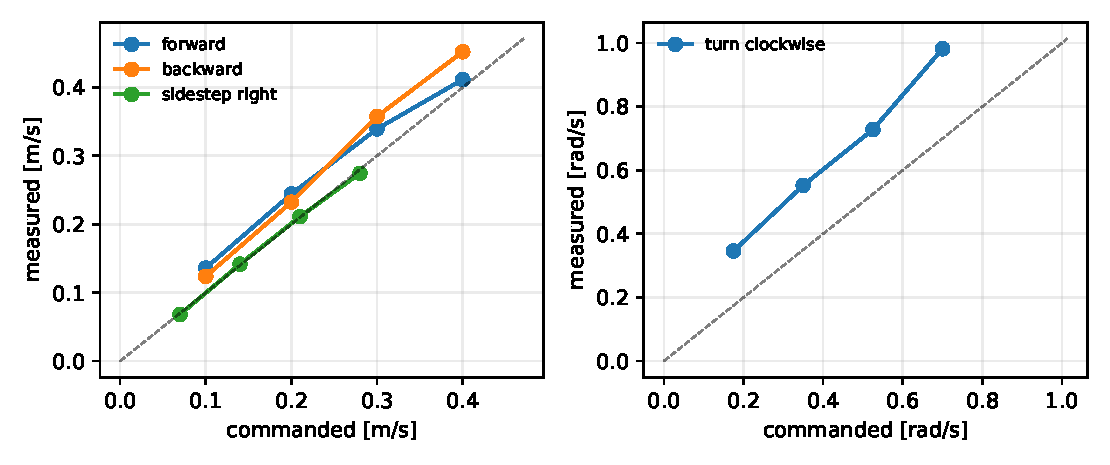
\includegraphics[width=0.7\linewidth]{figures/duck_ios_stick.pdf}
\caption{Measured against commanded velocity per stick axis. Dashed: equal.}
\end{figure}

\begin{table}[h]\centering
\begin{tabular}{lrrrl}\toprule
axis & deflection & commanded & measured & unit \\\midrule
\iosStick
\bottomrule\end{tabular}
\caption{The data of the figure.}
\end{table}
Translation follows the stick within 0.05~m/s. Turning is proportional but about 0.2--0.3~rad/s faster than
commanded at every deflection, a property of the walk policy, not of the stick. Both sticks at once (forward-right
while turning clockwise), as $(v_x, v_y, \omega_z)$: \iosCombo.

\subsection{The app in the simulator}
\texttt{ios/tools/test.sh}: the app in the iPhone~17~Pro simulator (iOS~26), driven by XCUITest, against
\texttt{studio.py --mock --lan} (a simulated bus of 15 servos, one of them on a factory ID, and simulated sensors)
and \texttt{server.py --lan} (the real engine and exports). The suite runs once in light and once in dark
appearance, then once with both servers stopped and restarted. The app is launched with \texttt{-mockOnly 1}, which makes it ignore any real studio, and every test that
touches servos first asserts that the studio is a mock: these tests switch torque and write zeros. Every assertion reads back what the servers did
through the app's accessibility values; in Play that is the trunk's world position and heading after a reset to
the origin.

\begin{table}[h]\centering
\begin{tabular}{lrrlr}\toprule
quantity & mean & range & unit & runs \\\midrule
\iosTable
\bottomrule\end{tabular}
\caption{Measured through the UI at speed level 3; each stick push is 3~s, each turn 1.5~s (a 3~s turn passed 180$^\circ$ and wrapped), and the pose is read once the duck stands
still again. Left is $+y$, anticlockwise is positive.}
\end{table}

What the tests establish:
\begin{itemize}\itemsep0pt
\item \textbf{Top bar.} Both servers are found over Bonjour; the switches bring the bus (14/15 joints plus the
factory-ID servo, all on screen without scrolling) and the duck's computer up and down; with both off, one tap on
Connect brings both back; Duck/Sim switches the screen, and Play on the real duck in Setup offers Run.
\item \textbf{Temperature.} The bar reads the mock's 41~$^\circ$C with no warning; the panel shows 41~$^\circ$C for the
processor and a hottest servo between 31 and 35~$^\circ$C.
\item \textbf{Battery, mode.} The battery percentage appears with the bus; Setup/Run switches and switches back;
Calibrate is disabled with 14 of 15 servos.
\item \textbf{Flip.} After a calibration, five nudges give a non-zero angle; Flip changes its sign and Flip again restores it.
\item \textbf{Calibration.} With the mock given its missing ID: Calibrate makes every servo limp, Hold holds them,
three nudges move the joint 6 ticks, Test and Zero are hidden meanwhile, Save reports success and the card then
reads 0.0$^\circ$; a second calibration is cancelled without effect.
\item \textbf{Servo.} Samples keep arriving; torque on; the slider at 0.8, 0.2 and 0.5 of its travel drives the
goal to three ordered positions more than 300 ticks apart; two nudges move it 4 ticks; Test swings the joint and releases it; gains 32/40 are read, 5/20 filled, written and
read back; Zero asks, then the pose reads 2048.
\item \textbf{Sensors.} Camera, ToF, IMU and microphone each show a reading; the IMU is calibrated from two poses and turned; two voice sounds play.
\item \textbf{Play.} Each stick direction moves the duck the right way (table); a half push covers less than a
full one; the duck stops when the stick is released; sit, stand, jump, flip and an emotion each pass through
their state and return to standing.
\item \textbf{Offline.} With nothing on the network Connect searches and then says ``Duck can't be reached''; the
panel's Host row reads ``Searching\ldots'' or ``Not found''. No command, path or flag is shown anywhere (the test
fails on any on-screen text containing one). When the servers start the app connects without being relaunched. The message came 4.0 and 4.4~s after the tap in the two runs measured.
\end{itemize}
Two things the table shows that are not the app's doing: a pure sidestep also turns the duck (tens of degrees in
3~s), and a straight push drifts in heading. The command carries no heading hold. On the engine alone, a full
forward command for 3~s from six different start phases ended at a heading of $-8$ to $13^\circ$ and 0.05 to
0.26~m to the side with the idle-life layer off, and $-41$ to $1^\circ$ and $-0.34$ to 0.30~m with it on (its
default), so most of the drift comes from that layer. An earlier run of this suite failed on a 0.35~m sideways
limit for that reason; the test now requires only that the duck ends further ahead than sideways.

\begin{figure}[h]\centering
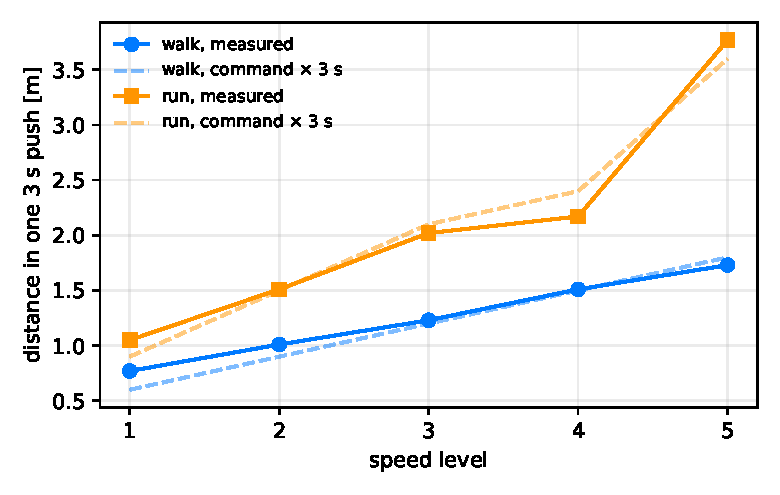
\includegraphics[width=0.7\linewidth]{figures/duck_ios_drive.pdf}
\caption{Distance ahead after one 3~s full forward push, per speed level, run switch off and on (one push each).
Dashed: the level's commanded speed times 3~s. Level 5 with run on is the sprint policy.}
\end{figure}

\begin{table}[h]\centering
\begin{tabular}{crrrr}\toprule
level & walk cmd [m/s] & walk dist. [m] & run cmd [m/s] & run dist. [m] \\\midrule
\iosDrive
\bottomrule\end{tabular}
\caption{The data of the figure.}
\end{table}

\subsection{Connection to the real duck}
\texttt{ios/tools/test\_connect.sh} cold-launches the app in the simulator against the real duck on the Wi-Fi
(read-only: the app opens the servo bus and reads; no servo command is sent), with the remembered address cleared
before every launch, seven times for each way of finding it alone and for all three together
(2026-11-18, duck at \texttt{radxa-zero3.local}, same /24 as the Mac).
\begin{table}[h]\centering
\begin{tabular}{lccc}\toprule
finding by & ok & found [s] & connected [s] \\\midrule
all three & 7/7 & 3.67 (3.60..3.84) & 5.46 (3.65..15.99) \\
Bonjour alone & 7/7 & 3.60 (3.54..3.69) & 3.64 (3.58..3.73) \\
name alone & 7/7 & 3.60 (3.56..3.65) & 3.64 (3.61..3.69) \\
sweep alone & 7/7 & 6.28 (3.93..20.03) & 6.32 (3.97..20.07) \\
\midrule outage: noticed, back & 4/4 & 2.0 (1.2..2.4) & 22.7 (22.2..23.1) \\
\bottomrule
\end{tabular}
\caption{Time from launch (including about 3.5~s of app start under XCUITest) to the duck found, and to its
computer and servo bus connected with no tap, as mean (range). Last row: the duck's server stopped for 8~s under a running app
(4 runs): time to notice, then time until found and connected again.}
\end{table}
\begin{figure}[h]\centering
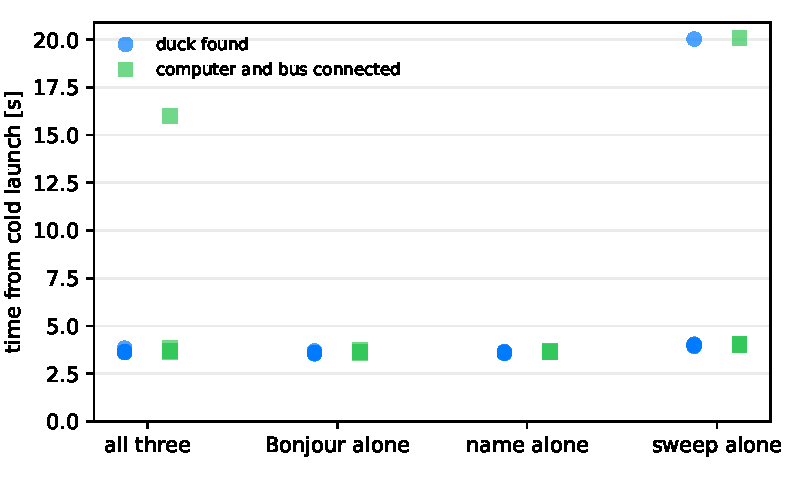
\includegraphics[width=0.7\linewidth]{figures/duck_ios_connect.pdf}
\caption{Every trial of the table.}
\end{figure}
All 28 launches found and connected. Two were slow: one sweep-only launch took 20~s (the first sweep missed the
duck and the next one runs 15~s later), and one launch took 16~s to connect after finding the duck in 3.6~s. The
second is the servo bus, not the network: during these runs \emph{no servo answered} (0 of 15, no battery
reading), and with nothing answering the studio's scan takes 11.7~s to open the bus (measured directly, one call).
The same 11.7~s is most of the 22.7~s recovery in the last row (8~s of outage, then the scan). With servos
answering the scan should be much shorter; that was not measured. The phone itself was not driven by a test.

\subsection{Play on the real duck's own policies, against a stand-in duck}
\texttt{ios/tools/mock\_studio.py} runs the mock studio unchanged and gives its mock duck what the real bridge
adds. The pilot is the duck's own code (\texttt{duck\_pilot.py}) with the real policy pack, ticked at 50~Hz, but fed
a still, upright IMU and joints at the default pose: states, speed levels, slew and timings are real, balance and
falls are not modelled, and nothing moves. Its commanded velocity is integrated into a planar pose so that a test
can see which way a stick sends it. Animations keep only the clock. The refusals are the bridge's, in its words.
The UI test \texttt{testPilot} tries power on an uncalibrated duck (refused), plays and stops animations, powers
on, pushes each stick, changes the speed level, runs, sits and stands, jumps, flips, leaves and re-enters Play, and
lets go. \texttt{testSensors} does the two-pose IMU calibration and the turns (the mock duck is ``laid on its
back'' after step 1).
\begin{table}[h]\centering
\small\begin{tabular}{@{}lcl@{}}\toprule
quantity & measured & expected \\\midrule
pilot runs, power on to let go & 2 & control loop 49.9 Hz \\
pushes of a stick & 12 & each ended by a zero command \\
gap between commands while held [ms] & 104 (48..171) & 100 (n = 230) \\
longest gap while held [ms] & 171 & under the pilot's 500 \\
command zero after release [s] & 0.27 (0.13..0.48) & n = 12 \\
a jump lasts [s] & 0.44 (0.44..0.44) & n = 2 \\
a flip lasts [s] & 0.98 (0.98..0.98) & n = 2 \\
sitting down [s] & 0.98 (0.97..0.98) & n = 2 \\
standing up [s] & 0.98 (0.98..0.99) & n = 2 \\
emotion tapped to playing [s] & 0.57 (0.54..0.61) & (n = 2) \\
``Hello'', tap to over [s] & 4.69 (4.51..4.87) & 3.5 + status lag (n = 2) \\
Start tapped to Standing shown [s] & 0.95 (0.92..0.97) & (n = 2) \\
forward, level 3, 3 s push [m] & 1.21 (1.19..1.22) & 1.20 = 0.40 m/s $\times$ 3 s (n = 2) \\
to the right, level 3, 2 s push [m] & 0.56 (0.56..0.57) & 0.56 = 0.28 m/s $\times$ 2 s (n = 2) \\
clockwise, level 3, 1 s push [deg] & 42.00 (42.00..42.00) & 40 = 0.70 rad/s $\times$ 1 s (n = 2) \\
forward, level 1, 2 s push [m] & 0.40 (0.39..0.40) & 0.40 = 0.20 m/s $\times$ 2 s (n = 2) \\
forward, level 5, 2 s push [m] & 1.22 (1.22..1.23) & 1.20 = 0.60 m/s $\times$ 2 s (n = 2) \\
running, level 3, 2 s push [m] & 1.50 (1.49..1.51) & 1.40 = 0.70 m/s $\times$ 2 s (n = 2) \\
\bottomrule
\end{tabular}
\caption{Play with the real duck selected, in Setup, on the stand-in duck; mean (range) where there are several
values. Distances are the stand-in's integrated pose over one push of the stated length. Times read through the
app include the studio's once-a-second status.}
\end{table}
\begin{figure}[h]\centering
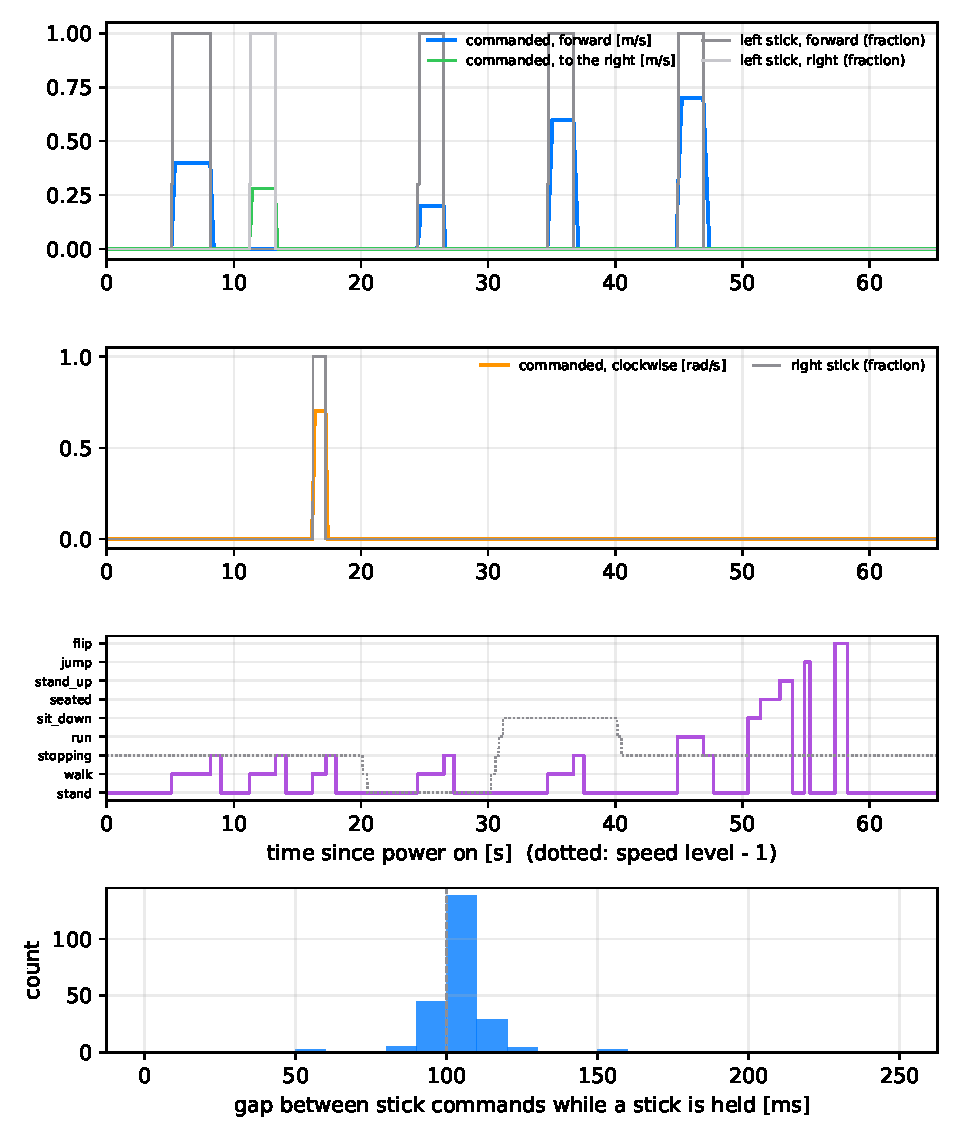
\includegraphics[width=0.7\linewidth]{figures/duck_ios_pilot.pdf}
\caption{One run of \texttt{testPilot}, power on to let go: the sticks as the pilot received them and the velocity
it commanded, its state and speed level, and the gaps between stick commands while a stick was held.}
\end{figure}

In the last full run both passes (light, dark) of \texttt{testPilot} passed. Sticks arrived 104~ms apart on
average while held (48 to 171, $n = 230$), and the pilot's command was back at zero 0.27~s after a release (0.13 to
0.48, $n = 12$), which is its own slew. Distances match the level's speed times the push to within 0.1~m.

\textbf{On the real duck} (2026-11-18, one read of the duck's studio state, nothing sent): Setup, 15 of 15 servos,
joints calibrated, IMU calibrated from two poses, 27 animations held, no pilot run in progress. So the fields the
app reads are there; whether the policy pack is on the duck was not asked.

\subsection{Play on the real duck, against a stand-in runtime}
\texttt{ios/tools/mock\_runtime.py} speaks the console's messages and models only what checks the app's commands:
unpowered until \texttt{robot.init} (a 2~s ramp), walking only after \texttt{robot.enable}, the applied velocity
following the requested one through the daemon's documented smoothing ($c \leftarrow c + 0.2\,(r - c)$ at 50~Hz)
within the limits above and integrated into a planar pose, and a 0.5~s deadman. No servo and no policy is involved,
so this tests the phone's side of the protocol, not the duck's walking. The UI test \texttt{testRunPlay} switches
the Mode to Run, taps power and walk, pushes each stick, changes the speed level, runs a skill, leaves and re-enters Play, and lets go.
\begin{table}[h]\centering
\small\begin{tabular}{@{}lcl@{}}\toprule
quantity & measured & expected \\\midrule
pushes of a stick & 11 & each ended by a zero command \\
gap between commands while held [ms] & 105 (50..192) & 100 (n = 190) \\
longest gap while held [ms] & 192 & under the 500 deadman \\
applied speed under 0.01 after release [s] & 0.38 (0.17..1.41) & n = 11 \\
Run tapped to runtime answering [s] & 1.42 (1.41..1.44) &  (n = 2) \\
power tapped to Standing [s] & 2.41 (2.35..2.48) & 2.0 ramp (n = 2) \\
forward, level 3, 3 s push [m] & 0.53 (0.53..0.53) & 0.54 = 0.18 m/s $\times$ 3 s (n = 2) \\
to the right, level 3, 2 s push [m] & 0.35 (0.34..0.36) & 0.36 = 0.18 m/s $\times$ 2 s (n = 2) \\
clockwise, level 3, 1 s push [deg] & 52.50 (52.00..53.00) & 52 = 0.9 rad/s $\times$ 1 s (n = 2) \\
forward, level 1, 2 s push [m] & 0.12 (0.11..0.13) & 0.12 = 0.06 m/s $\times$ 2 s (n = 2) \\
forward, level 5, 2 s push [m] & 0.58 (0.58..0.59) & 0.60 = 0.30 m/s $\times$ 2 s (n = 2) \\
\bottomrule
\end{tabular}
\caption{Play with the real duck selected, on the stand-in runtime; mean (range) where there are several values.
Distances are the stand-in's integrated pose over one push of the stated length.}
\end{table}
\begin{figure}[h]\centering
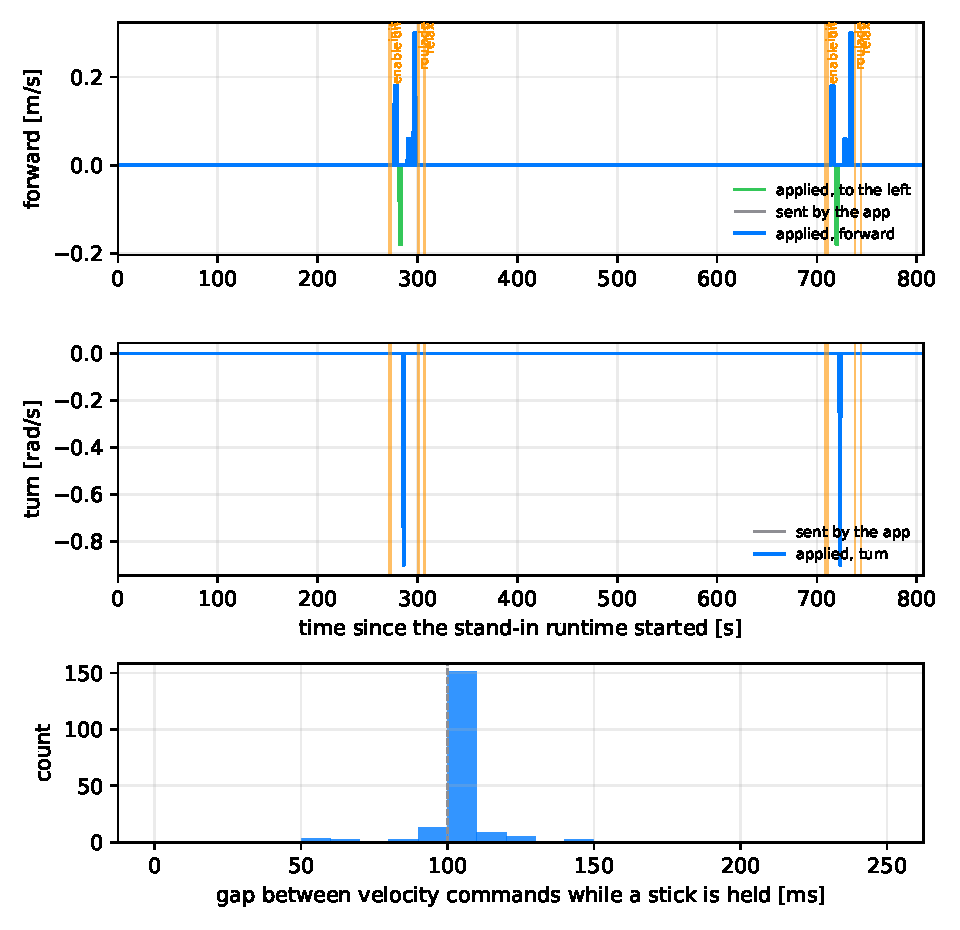
\includegraphics[width=0.7\linewidth]{figures/duck_ios_runtime.pdf}
\caption{One run of \texttt{testRunPlay}: the velocities the app sent and the stand-in applied, with the other
commands marked (orange), and the gaps between velocity commands while a stick was held.}
\end{figure}

\textbf{On the real duck} (2026-11-18, read-only, \texttt{ios/tools/runtime\_probe.py}: it never sends
\texttt{robot.init}, \texttt{robot.enable}, \texttt{robot.move} or a skill, so no joint was powered). Three reads:
\begin{enumerate}\itemsep0pt
\item Before the fixes: the console answered \texttt{hello} (API version 17, daemon 0.13.3) and listed its six
policies, but its health report said \emph{no robot on the motor bus} and it sent no state. The bridge was holding
the servo port, and a studio on the Mac then put the duck back in Setup (faults (i) and (ii) above).
\item With the bridge fixed but started by hand, the report was the same after 16 attempts, for a reason not
found (the daemon's log needs root). About a minute later the duck left the network and was back, rebooted,
18~minutes later; whether the two are related is not known. Its processor read 74~$^\circ$C shortly before.
\item After that reboot: Setup to Run took 0.36~s; the daemon reported \emph{healthy}, bus ok, IMU ready, the
loop at 50.0~Hz with 0 missed cycles, battery 7.93~V (83~\%), hottest servo 34~$^\circ$C, processor
83~$^\circ$C; the state stream arrived at 9.0~Hz (35 messages in 4~s, 10 asked for).
\end{enumerate}
The third read also corrected the app: an unpowered duck reads policy \texttt{held} with \texttt{limp} false
(and \texttt{fallen} true when lying down), so the state has no flag for ``joints powered''. The app therefore
takes power from its own accepted \texttt{robot.init} and \texttt{robot.relax}, and from a running policy
(walk, stand, sit/stand or a skill) when it finds the duck already up. The runtime's joint angles differed from
the studio's for the same resting pose by up to 96$^\circ$ (right knee: $-79.4^\circ$ against $16.3^\circ$), which
is why they are not drawn.

\subsection{Camera and microphone decoding}
\texttt{ios/tools/check\_codec.py} compiles the app's own decoder (\texttt{Duck/Pixels.swift}) for the Mac and
compares it with an independent floating-point NV12 decoder (full range, BT.601, which is what the duck's ISP
reports) on synthetic frames and on frames just taken from the real duck.
\begin{table}[h]\centering
\begin{tabular}{llrrr}\toprule
frame & size & max $|$err$|$ & mean $|$err$|$ & pixels off [\%] \\\midrule
colour bars & $320\times 240$ & 0 & 0.000 & 0.0 \\
luma ramp & $320\times 240$ & 0 & 0.000 & 0.0 \\
chroma ramps & $320\times 240$ & 1 & 0.000 & 0.0 \\
noise (seed 0) & $320\times 240$ & 1 & 0.000 & 0.0 \\
noise, 64x48 & $64\times 48$ & 1 & 0.000 & 0.0 \\
real duck, frame 1 & $320\times 240$ & 1 & 0.000 & 0.0 \\
real duck, frame 2 & $320\times 240$ & 0 & 0.000 & 0.0 \\
real duck, frame 3 & $320\times 240$ & 1 & 0.000 & 0.0 \\
real duck, frame 4 & $320\times 240$ & 1 & 0.000 & 0.0 \\
\bottomrule
\end{tabular}
\caption{App decoder against the reference, in 8-bit levels per channel.}
\end{table}
\begin{figure}[h]\centering
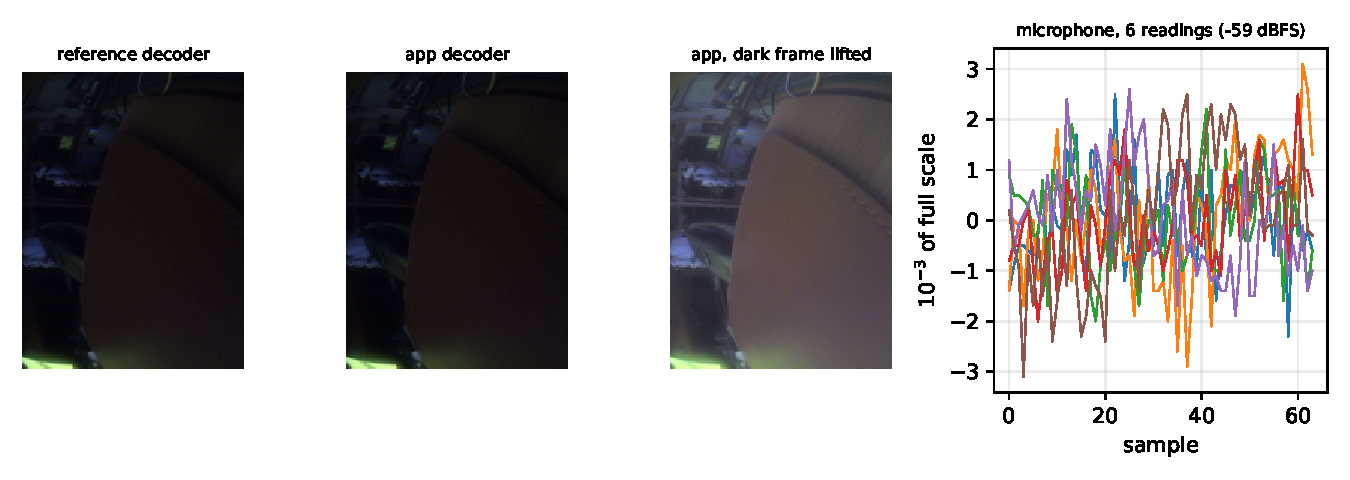
\includegraphics[width=0.7\linewidth]{figures/duck_ios_codec.pdf}
\caption{A frame from the real duck: reference, app, app with the dark-frame lift; and six microphone readings.}
\end{figure}
The decoder is correct to one level (single- against double-precision rounding). The picture the duck sent was
very dark (mean luma about 20 of 255, sensor gain already at its maximum), which on the phone looked like no
picture. The app now lifts a dark frame: with mean luma $\bar{y}$ below 89, luma is mapped
$y' = 255\,(y/255)^{\gamma}$ with $\gamma = \max(0.45, \ln 0.35/\ln(\bar{y}/255))$, and chroma is scaled by
$\min(2, \sqrt{y'/y})$. The check confirms the map is monotonic, never darkens, and leaves frames with
$\bar{y}\ge 90$ untouched. It also amplifies sensor noise, and $\gamma$ is recomputed per frame with no smoothing.
The microphone's readings were consistent (64 samples, level equal to the samples' own RMS within 0.6~dB) but
small: $-59$~dBFS in a quiet room, peaks 0.004 of full scale, which the old fixed gain of 3 drew as a flat line.
The trace is now drawn against the loudest recent sample (decaying 10\,\% per reading, floor 0.002); in the
simulator against the real duck it then spanned 0.71 of the window on average (minimum 0.55, 20 readings). Only the
right channel and a quiet room were looked at; a loud sound was not tried.

Defects found by the tests and fixed: positions above 999 were printed with a thousands separator; the servo
card's bottom row was wider than the screen; the reset button only responded on the glyph's own pixels.

\begin{figure}[h]\centering
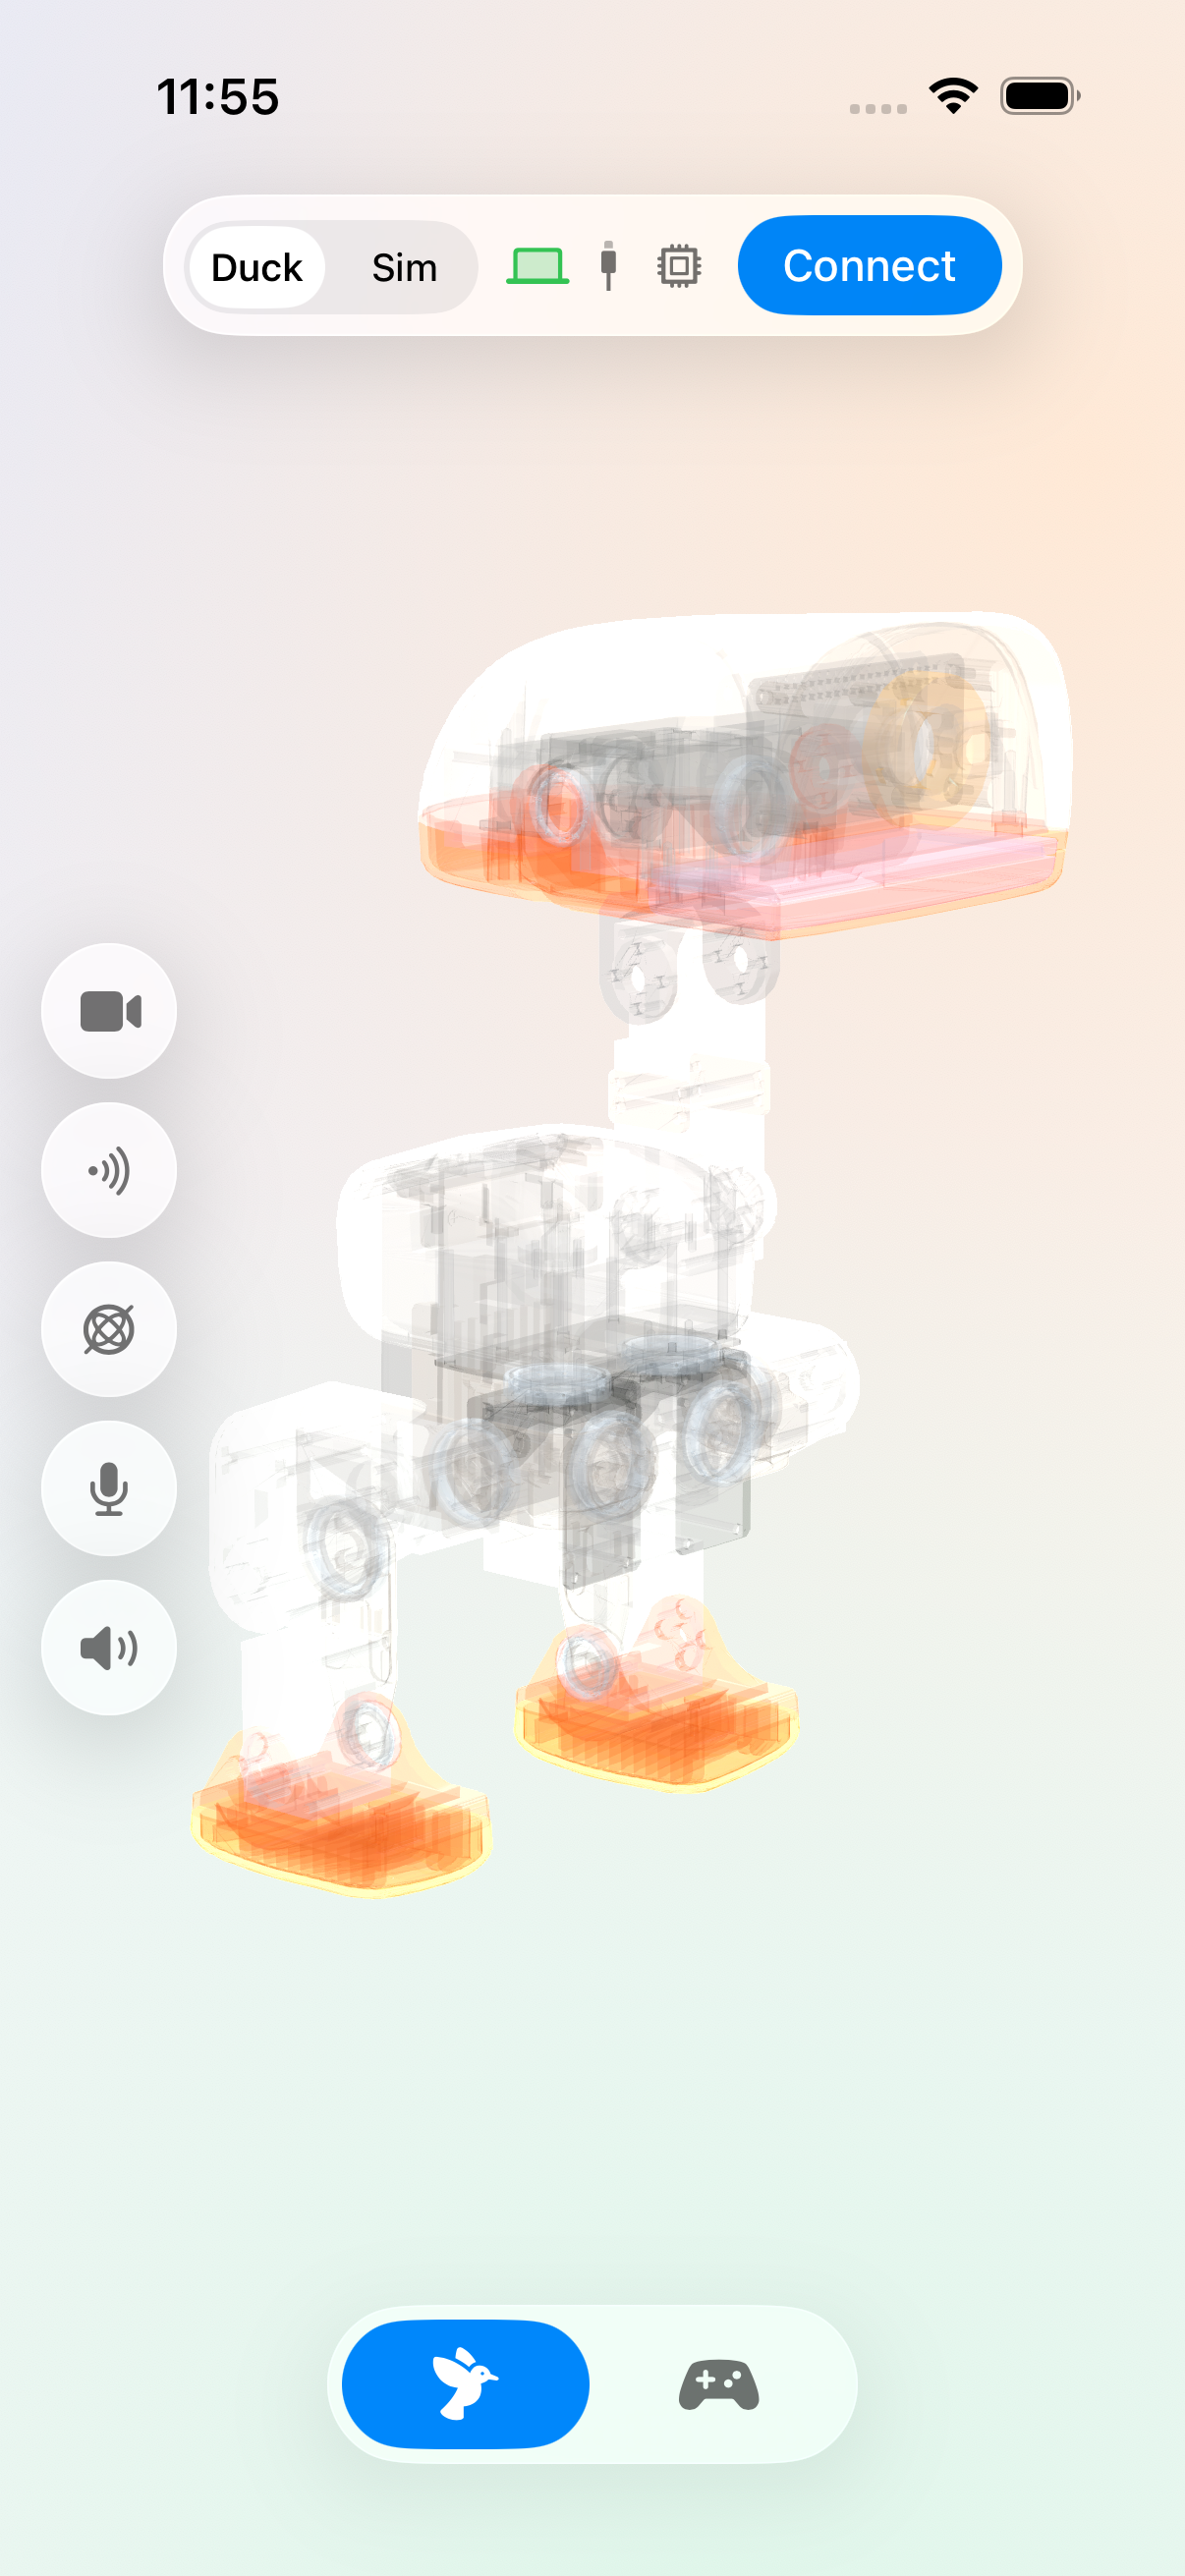
\includegraphics[width=0.23\linewidth]{figures/ios/03b_disconnected.png}\hfill
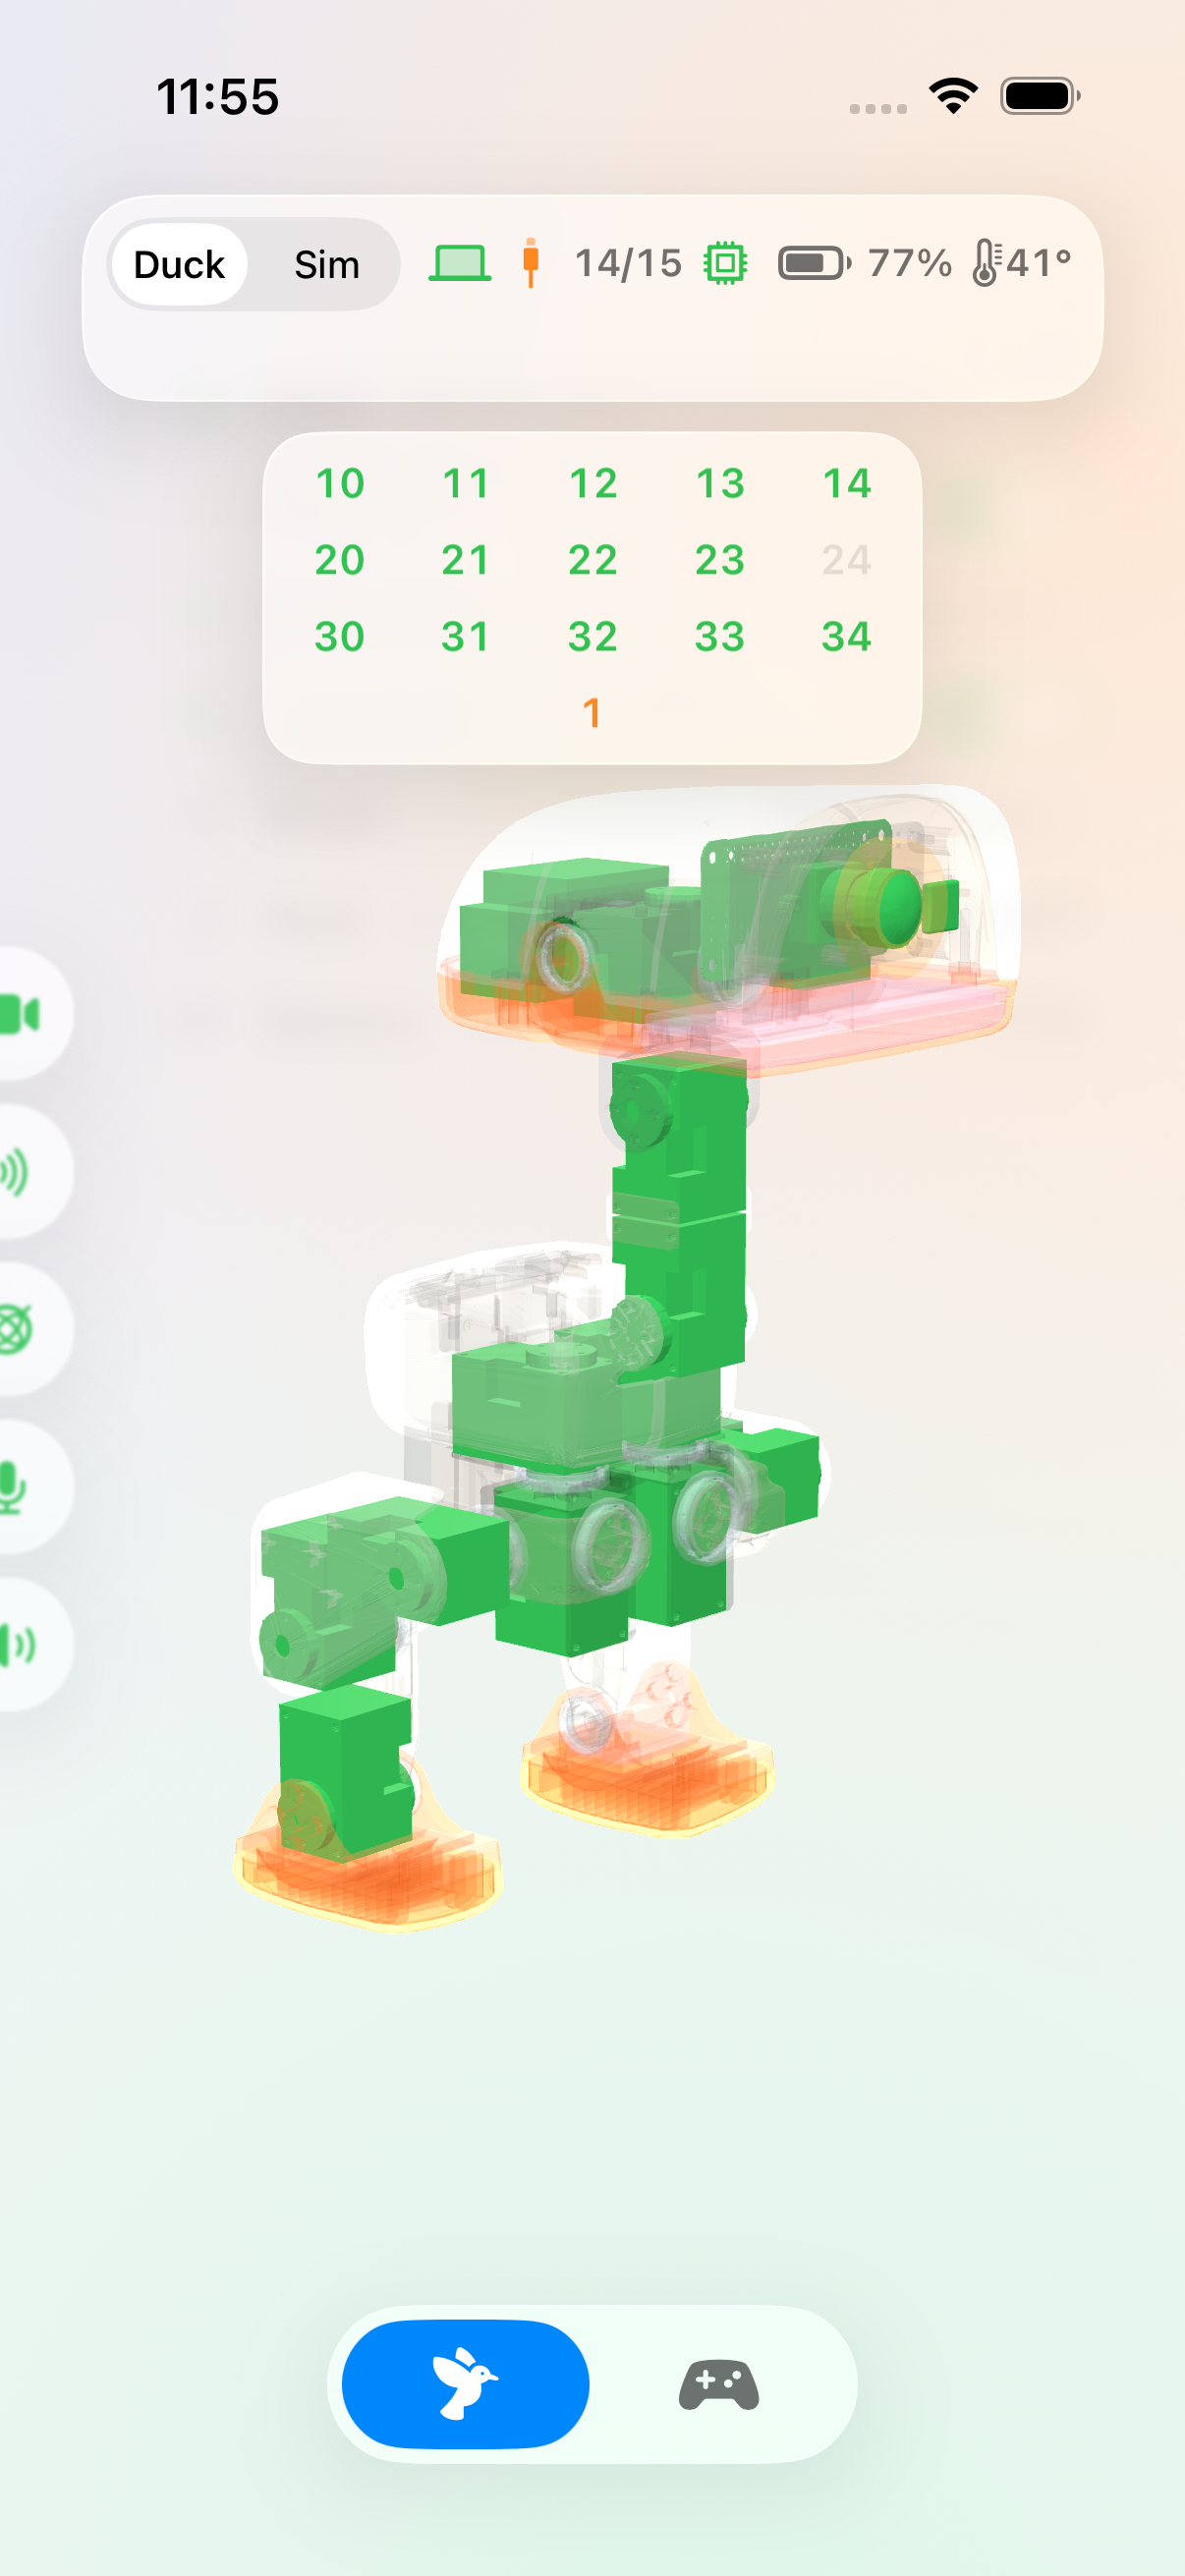
\includegraphics[width=0.23\linewidth]{figures/ios/03_connected.png}\hfill
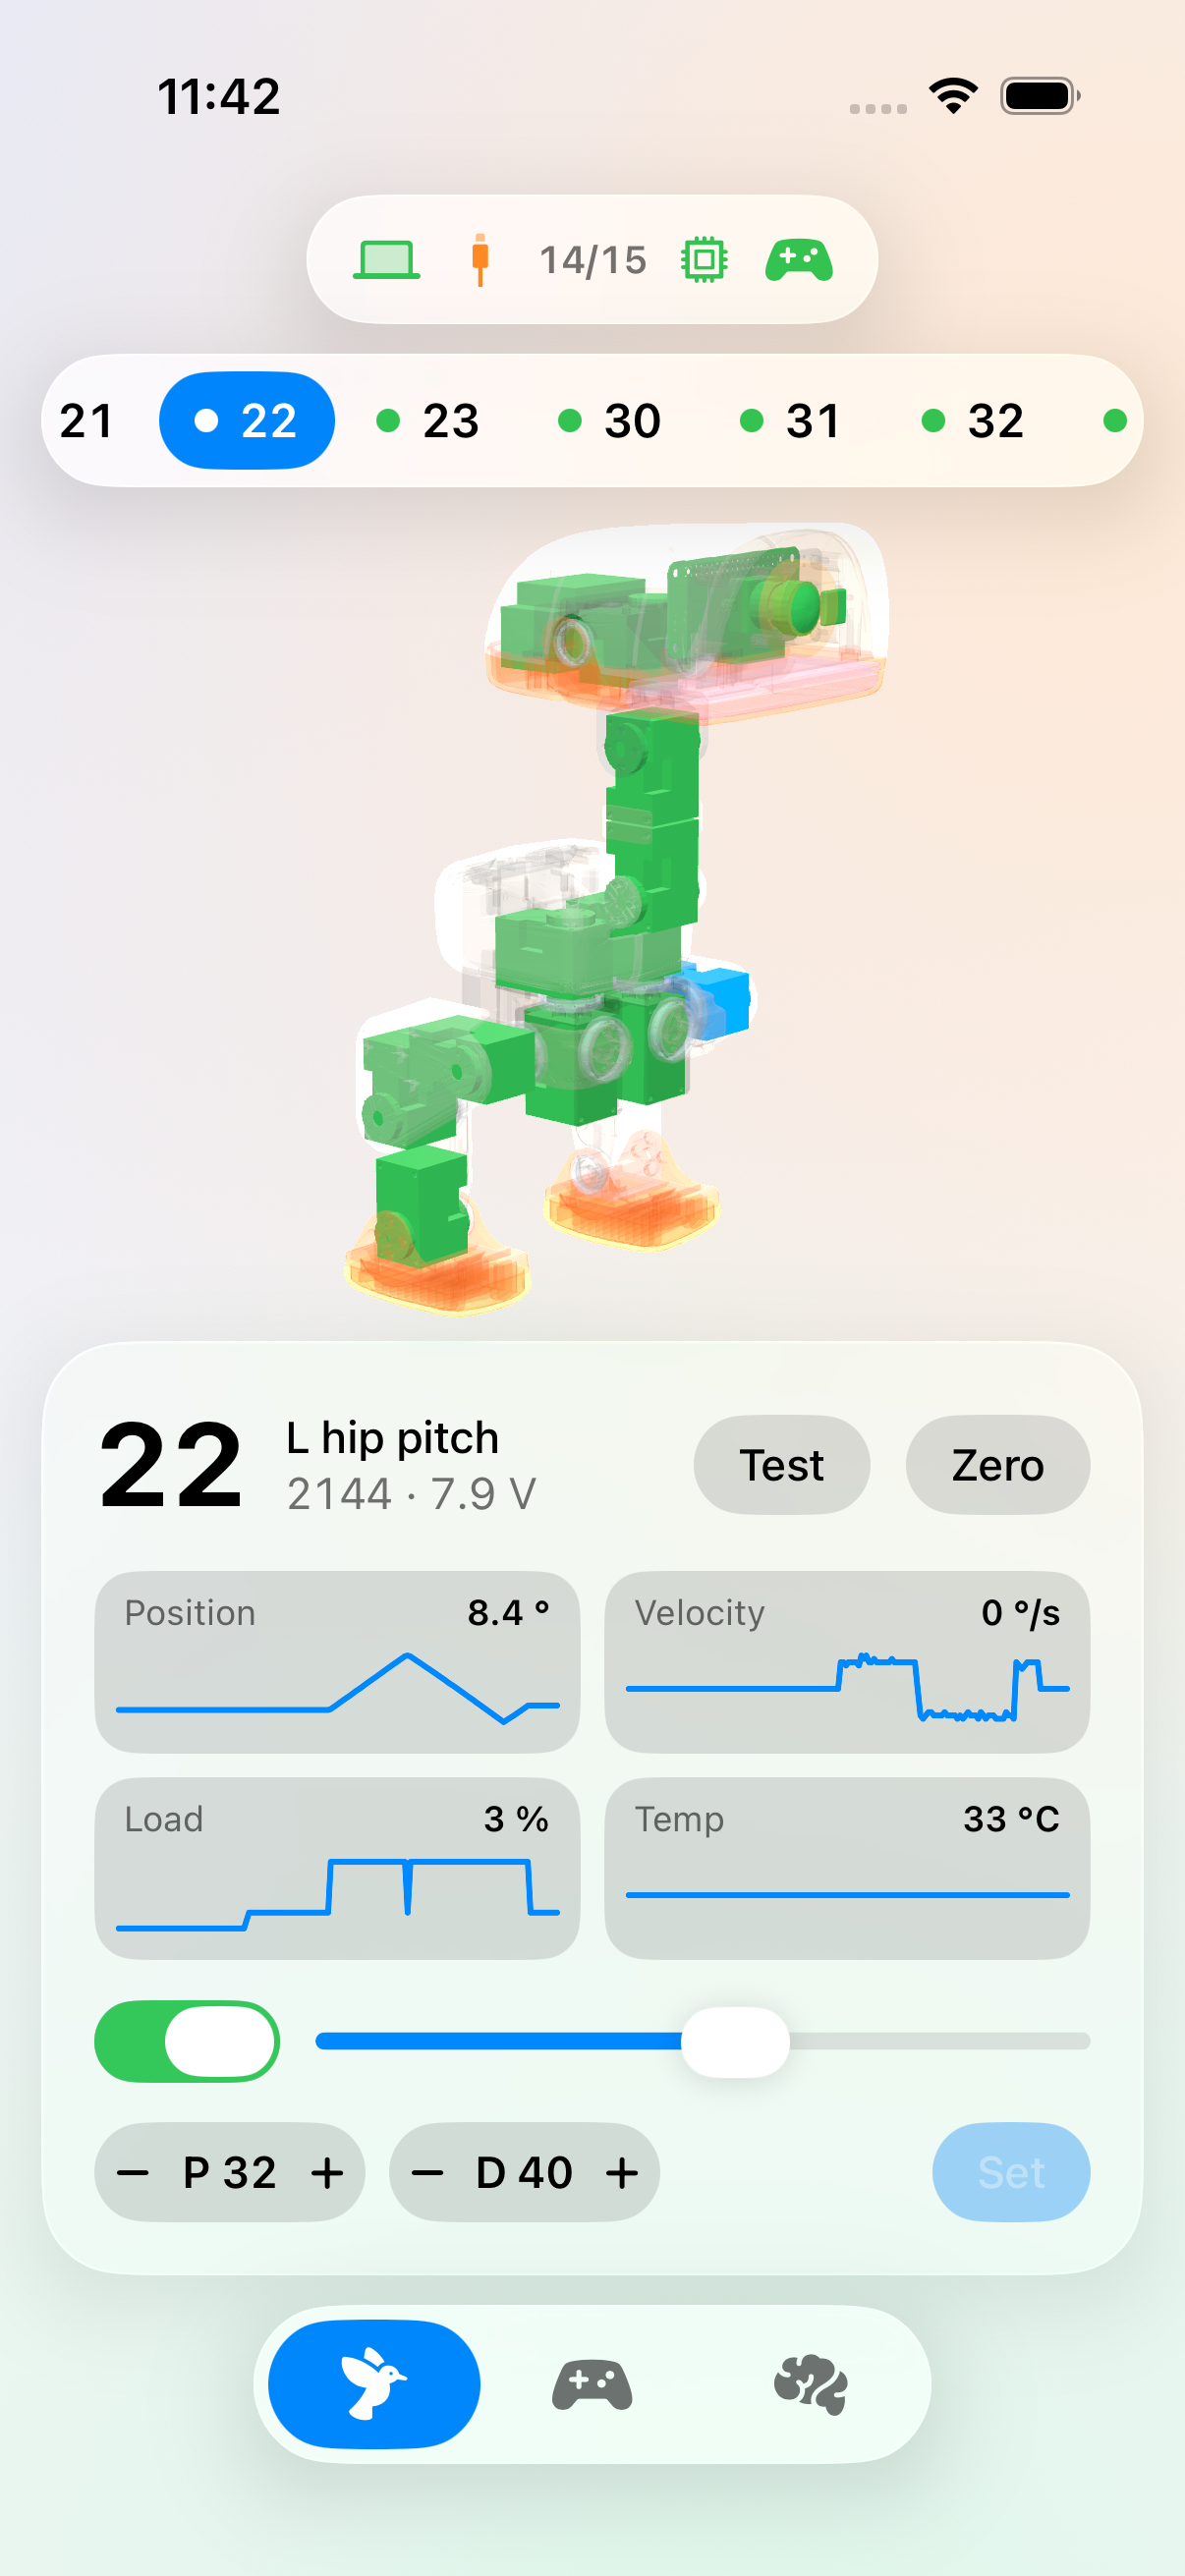
\includegraphics[width=0.23\linewidth]{figures/ios/04_servo.png}\hfill
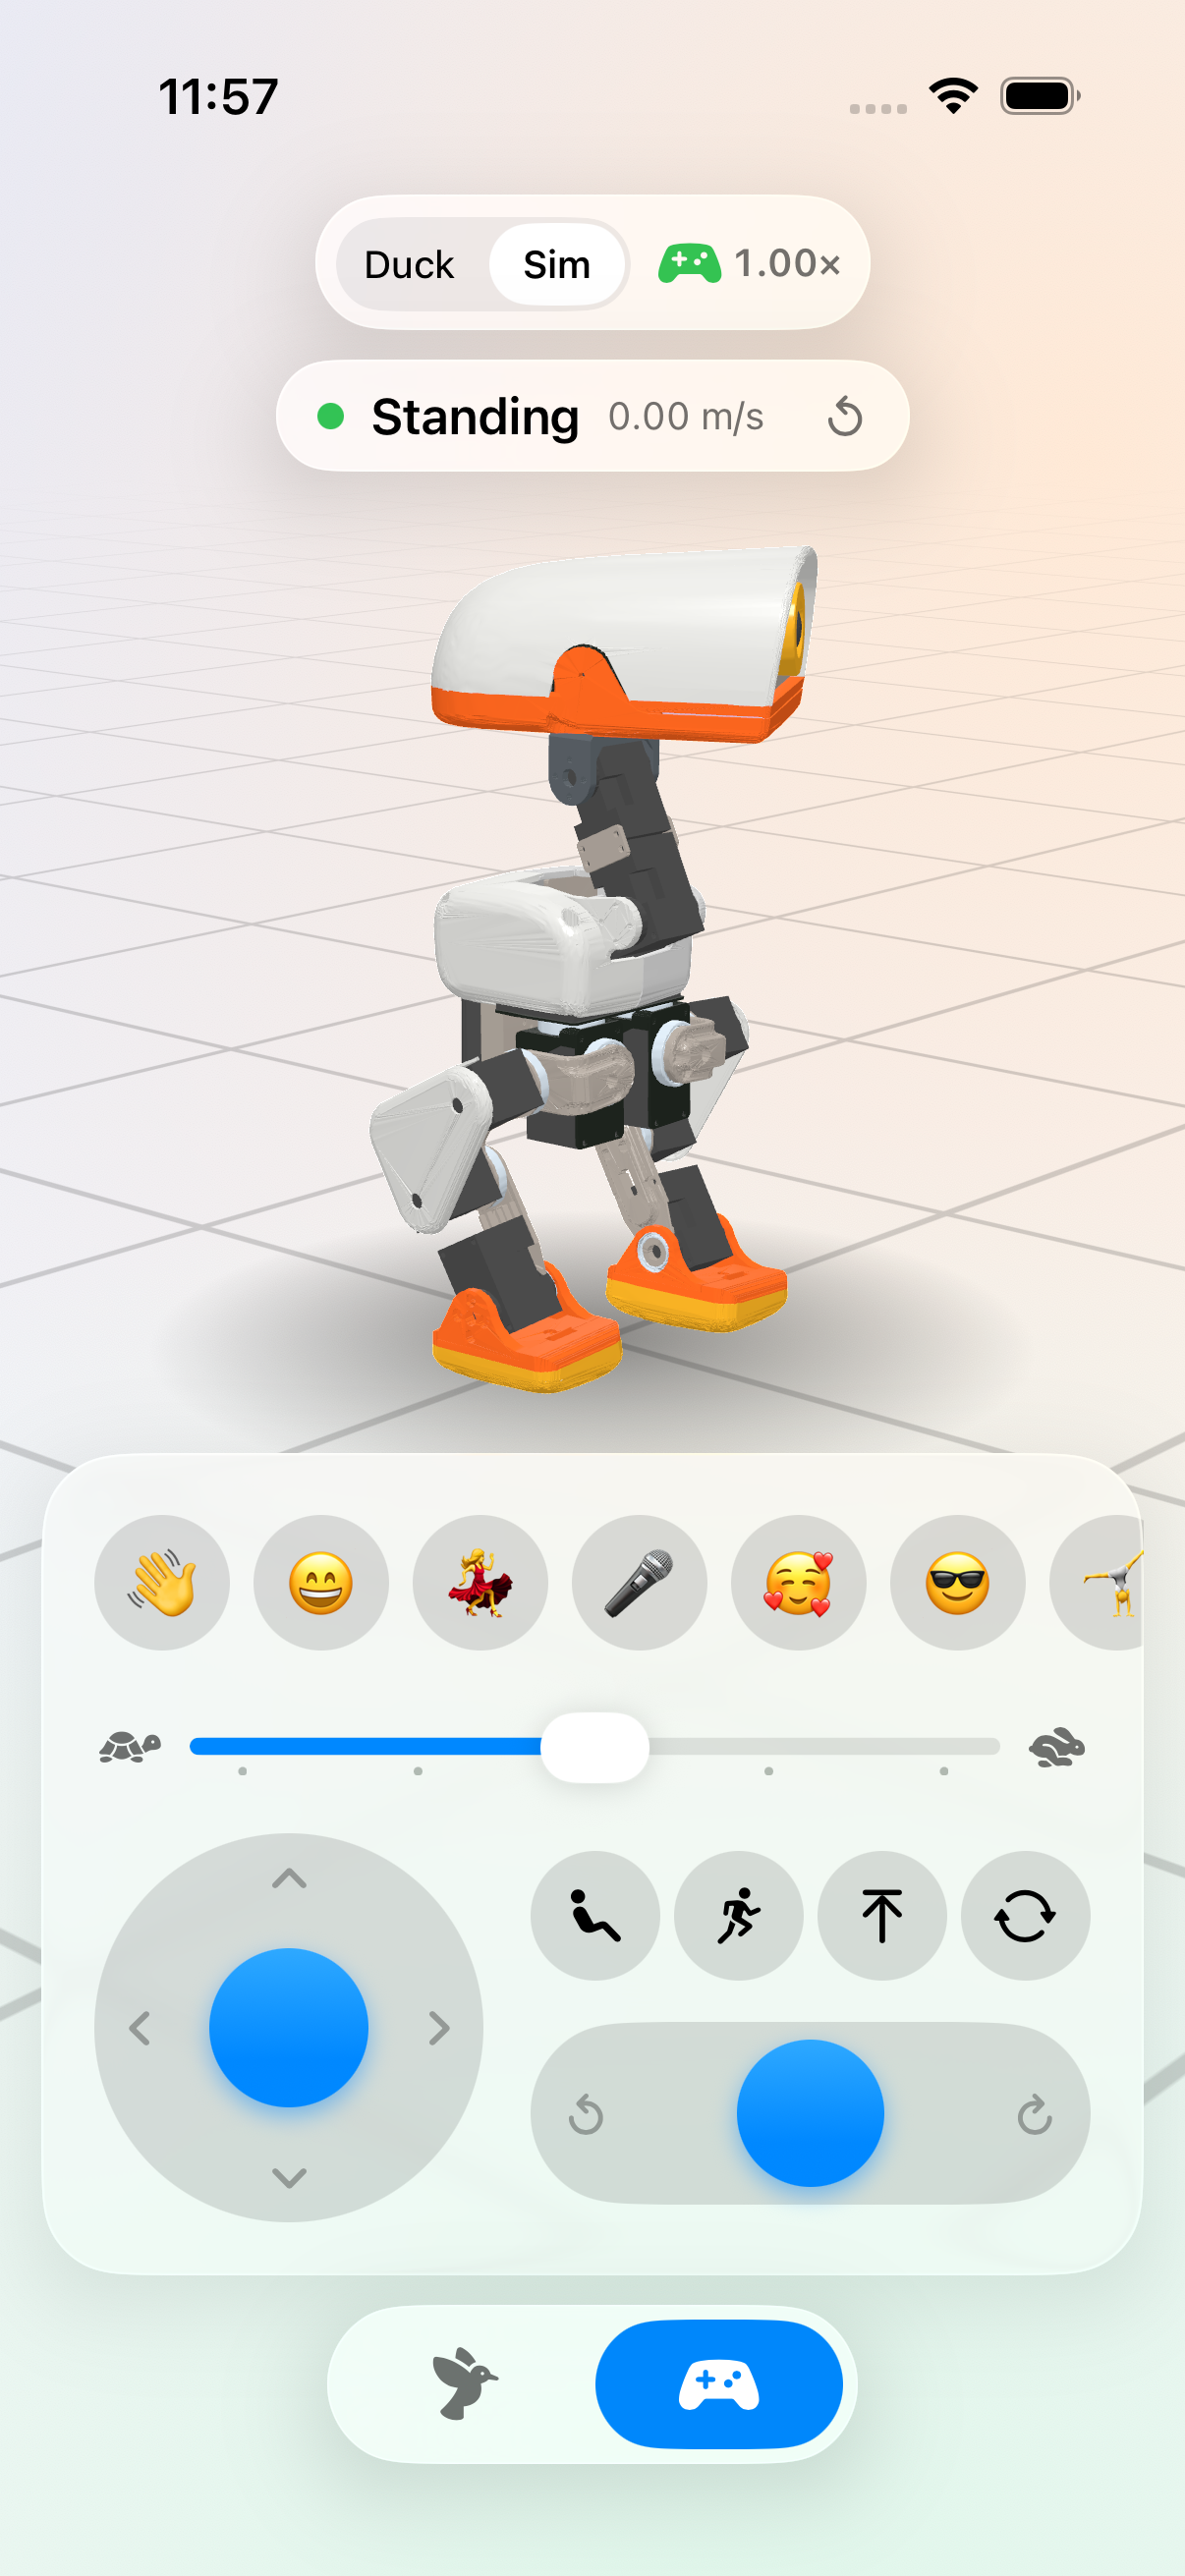
\includegraphics[width=0.23\linewidth]{figures/ios/07_play.png}
\caption{Real duck not connected, connected, a selected servo; Sim in Play (simulator screenshots written by the
tests).}
\end{figure}

\section{Implementation and usage}
\begin{verbatim}
firmware/studio.py --lan     # on the Mac (add --mock for no hardware)
app/server.py --lan
cd ios && DEVELOPMENT_TEAM=<team id> xcodegen generate && open Duck.xcodeproj
ios/tools/test.sh            # the whole simulator test
ios/tools/plot_tests.py      # figure and numbers from its log
ios/tools/bench_stick.py     # stick tracking on the engine
ios/tools/plot_pilot.py      # Play, the duck's own policies: figure, table
ios/tools/mock_studio.py     # the mock studio with a stand-in duck
ios/tools/plot_runtime.py    # Play, the factory runtime: figure, table
ios/tools/runtime_probe.py   # the real runtime, read-only
firmware/duck_serve.sh       # studio and bridge onto the duck
\end{verbatim}
\texttt{Link.swift} holds discovery and both clients in one observable model; \texttt{Scene.swift} the model
loader and SceneKit scene; \texttt{Views.swift} the screen. The hardware path is unchanged from the studio: the
phone speaks to \texttt{studio.py}, which owns the serial bus in Setup, and in Run to the runtime's console on
the duck (port 8090; beside a mock studio, the stand-in on 8791).

\section{Limitations}
\begin{itemize}\itemsep0pt
\item Simulator only. On the iPhone: local-network permission, Wi-Fi latency, touch feel, and two thumbs on both
sticks at once are untested (XCUITest drives one stick at a time; the combination is covered on the engine only).
\item \textbf{On the real duck:} on 2026-11-17 the duck dropped off the network minutes after the duck-side studio
was first started, with a last reported processor temperature of 110.6~$^\circ$C; the cause is not known. After a
reflash it ran through the tests above on 2026-11-18 at 75--79~$^\circ$C, which is already in the app's ``warm''
band; later that day it left the network once more for 18~minutes and came back rebooted, at 83--85~$^\circ$C. During the connection tests no servo and no IMU answered on the bus and the ToF gave no reading (another process held
it), so servos, battery, IMU and ToF were not seen on the real duck through the app.
\item The servo side was tested against the mock bus; on real servos the studio's own caveats apply
(\texttt{firmware/README.md}). Connect, calibration and Setup/Run were not tried against a real duck; a mock
studio does not write the calibration file.
\item \textbf{Play on the real duck has not moved the real duck.} Under its own policies (Setup): power, the
sticks, the moves and the animations are verified against the stand-in duck only, which cannot fall. From the phone
no clip was played and no policy started on the real duck. The state word is up to 1~s old. While the policies
drive, the Duck tab's servo cards still send their commands to the studio, as the studio page does; nothing in the
app stops a slider there from fighting the policy.
\item Under the factory runtime (Run): standing, walking, the skills and the stop on
release are verified against the stand-in only; on the real duck the app's path was checked as far as a healthy
runtime and its state stream. The policy names of a standing or walking duck (\texttt{stand}, \texttt{walk}, \ldots)
are taken from the daemon's policy list, not observed; if they differ, the state word and the walk light can be
wrong after reconnecting to a duck that is already up, though the commands are not affected. The left
kick has no policy installed on this duck; the runtime will refuse it.
\item Anyone on the network can drive the duck: the console on port 8090 has no login.
\item \texttt{--lan} gives everyone on the network access; the studio has no login and the engine's token is
readable in its Bonjour record.
\item Emotion sounds are not played on the phone.
\item One push or run per setting; the hold time is XCUITest's, not a calibrated timer.
\item The studio was being changed while this was built (its speaker route became \texttt{say}); the app matches
the studio as of this date.
\end{itemize}

\begin{thebibliography}{9}
\bibitem{pollen} Pollen Robotics, \emph{microduck} and \emph{microduck\_emotions}, GitHub, Apache-2.0.
\bibitem{mujoco} E.~Todorov, T.~Erez, Y.~Tassa, ``MuJoCo: A physics engine for model-based control,'' IROS 2012.
\bibitem{dnssd} S.~Cheshire, M.~Krochmal, ``DNS-Based Service Discovery,'' RFC~6763, 2013.
\bibitem{kissqy} kissqy, \emph{Microduck-kissqy}, GitHub (HD1910 replica: ID map, registers, gains).
\end{thebibliography}
\end{document}
